\documentclass{article}[18pt]
\usepackage{../../../../format}
\lhead{Computer Systems}


\begin{document}
\begin{center}
\underline{\huge Logic Gates and Transistors}
\end{center}

\section{Transistors}
A transistor is just an electronically controlled switch: 2 ports (d and s) are connected depending on the voltage of 3rd (g)\\
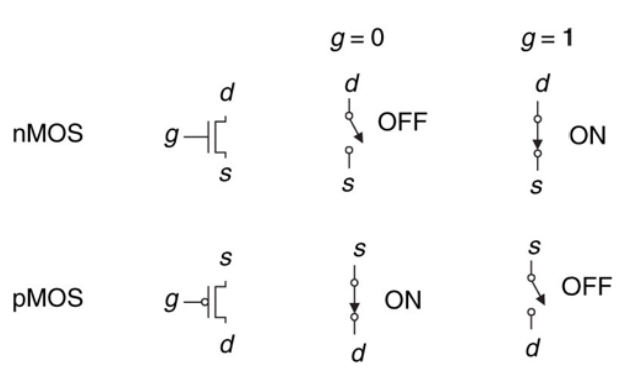
\includegraphics[width=10cm]{Fig1.png}\\
The most common transistor is the MOSFET (Metal Oxide Semiconductor Field Effect Transistor)\\
Silicon (a semiconductor) is a poor conductor of electricity: all the available electrons(4) are used to form bonds with neighbouring atoms\\
Impurities (dopants) provide extra electrons or electron holes which increase conductivity\\
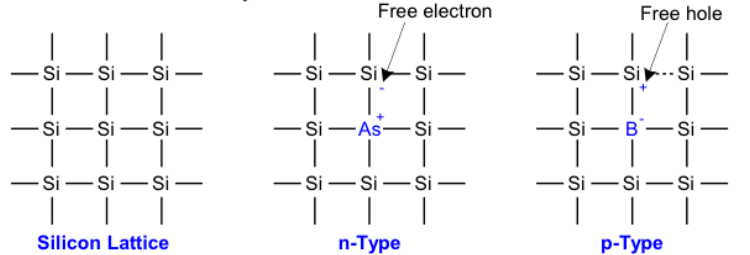
\includegraphics[width=10cm]{Fig2.png}\\
In n type silicon it has a negative charge overall as there is a free electron in the lattice\\
In p type silicon an additional electron is ripped from the silicon atom, causing the lattice to have an overall positive charge. This lack of an electron can float around in the substrate, and acts like a positive charge.\\
The n type is a more efficient carrier.
\subsection{Diodes}
At a junction between p-type and n-type silicon, current can only flow from p type to n-type. This is a diode.\\
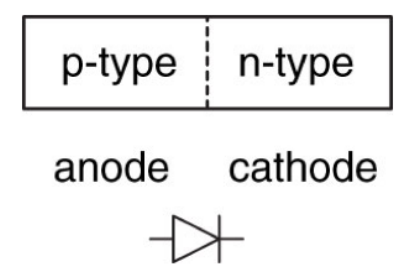
\includegraphics[width=6cm]{Fig3.png}
\begin{itemize}
\item Attach a negative charge near the p type, the holes will be attracted. This will cause a depleted region in the middle. A positive charge near the n type would pull the charge away from the middle. In this area in the middle current cannot flow.
\item Note that with enough voltage charge will be carried whatever way intended
\end{itemize}
\subsection{Capacitors}
A \textbf{capacitor} is two pieces of conductive material separated by an insulator\\
\\
If a positive voltage is applied to one side, it accumulates charge Q and the other side accumulates the opposite charge -Q.\\
\\
It takes time and energy to charge and discharge a capacitor
\begin{itemize}
\item The charges attract each other, and so is maintained when taken away
\item Applying a sufficiently high voltage at one end the electrons will be pulled in the intended way
\end{itemize}
\subsection{More detail about transistors}
\subsubsection{nMOS transistor}
\includegraphics[width=8cm]{NMOS.png}\\
When the gate g is at $V_{DD}$, the capacitor effect draws negative charge (electrons) to the surface, and create a temporary channel of n type silicon, which allows current to flow from source to drain
\begin{itemize}
\item In its natural state there is no conduction
\item By raising the gate voltage to a sufficiently high voltage a capacitance effect will be created between the gate and the p type substrate (rip electrons off atoms and pull through the substrate to create a layer of floating electrons between the source and drain.
\end{itemize}
\subsubsection{pMOS transistor}
A pMOS transistor is the opposite: on at g low and off at g high\\
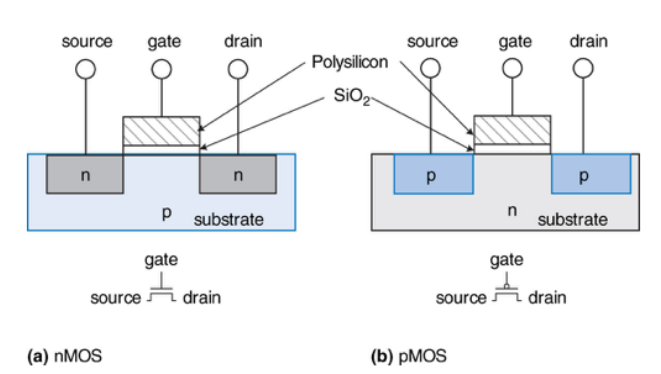
\includegraphics[width=8cm]{pMOS.png}
\begin{itemize}
\item This is the same design as the nMOS transistor, but with the doped silicon the other way round
\item The nMOS transistor is more efficient and so can be made slightly smaller
\end{itemize}
\newpage
\section{Binary Addition}
This is achieved using gates implementing boolean algebra\\
\\
Boolean algebra: An algebra of 2 values, 0 and 1\\
\\
Basic Operations
\begin{itemize}
\item 0 and 0=0
\item 0 and 1=0
\item 1 and 0=0
\item 1 and 1=1
\end{itemize}
\subsection{Truth Tables}
\subsubsection{AND}
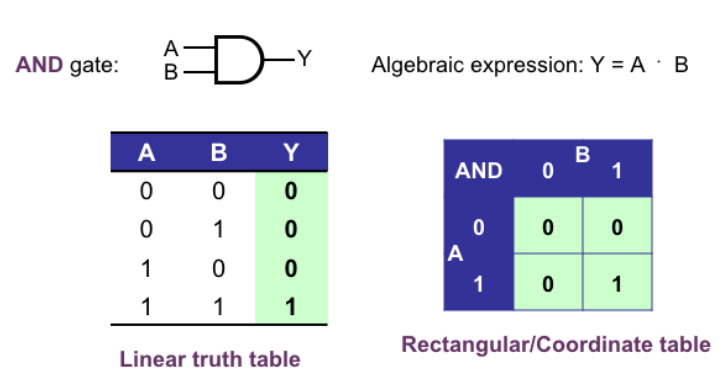
\includegraphics[width=8cm]{AND.png}
\subsubsection{OR}
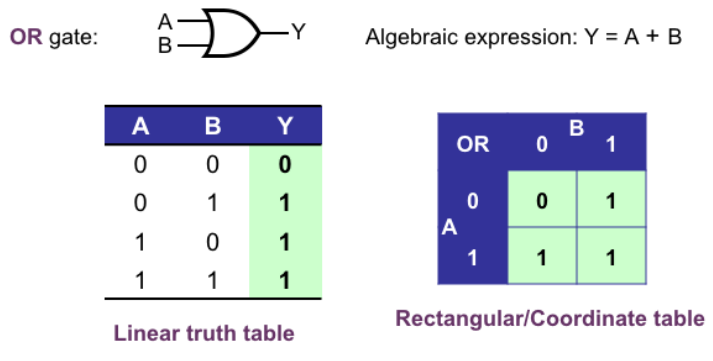
\includegraphics[width=8cm]{OR.png}
\subsubsection{NOT}
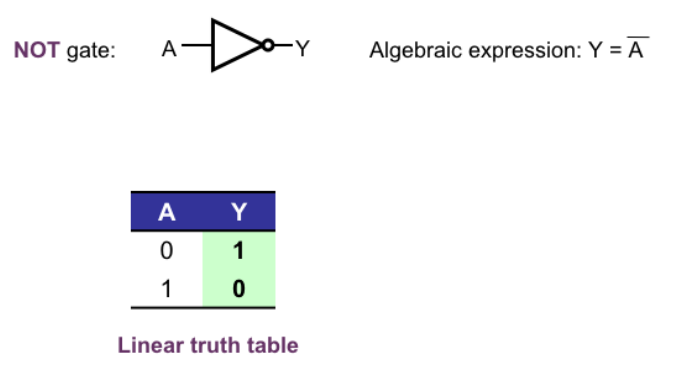
\includegraphics[width=8cm]{NOT.png}
\section{From transistors to gates}
\subsection{NOT}
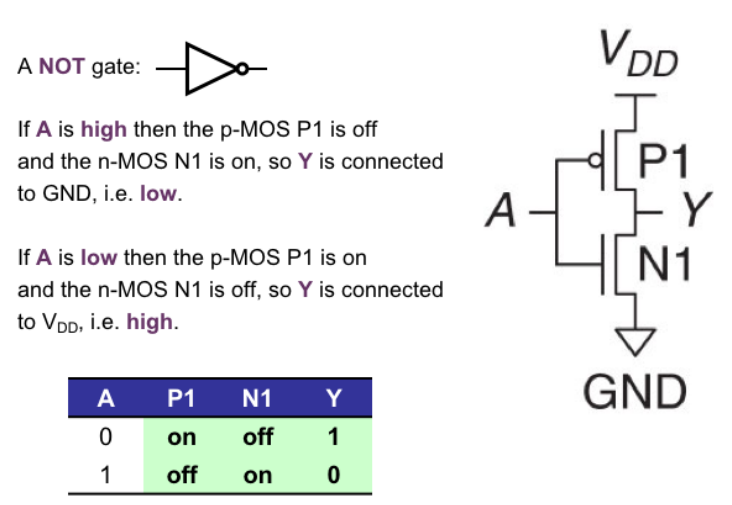
\includegraphics[width=15cm]{NOTTrans.png}
\subsection{NAND}
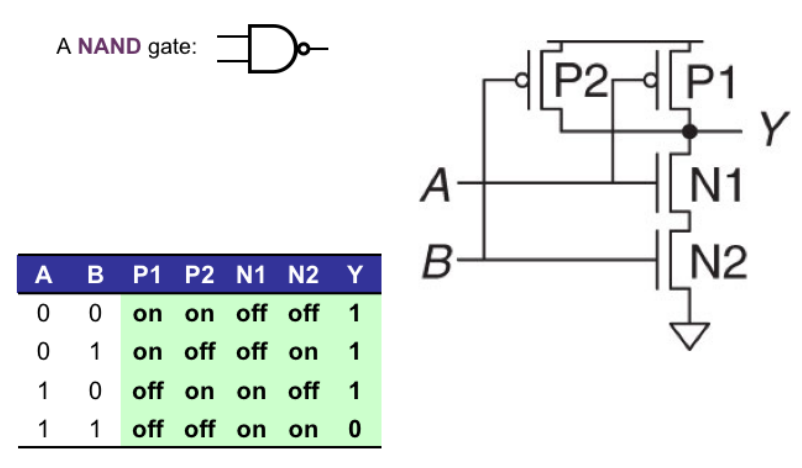
\includegraphics[width=15cm]{NANDTrans.png}
\section{Beneath the digital abstraction}
The chip does not really deal with 0s and 1s. The voltages are real numbers typically between 0V and 5V.\\
\\
We can take 0V to indicate output 0 and 5V to indicate output 1, but we need to tolerate \textbf{noise}. It is obvious if the value is close to one of the extremes, but what if it was 2.5V?
\section{Supply Voltage}
The low voltage in the system is 0V\\
\\
Historically the high voltage ($V_{DD}$) was 5V, but more modern transistors use lower voltages to save power and avoid overloading transistors\\
\\
The mapping of the continuous voltage measured at any point in the circuit to the discrete 0 and 1 of the digital abstraction is governed by defining \textbf{logic levels}
\subsection{Logic Levels}
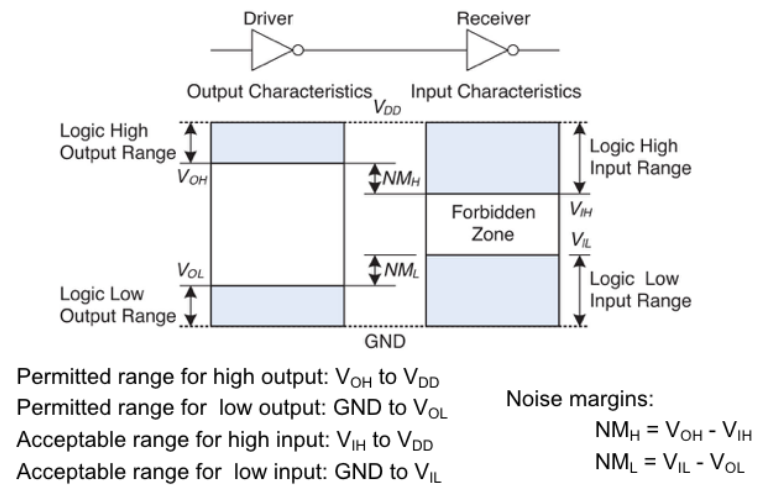
\includegraphics[width=15cm]{LogicLevels.png}
\begin{itemize}
\item It is best for logic levels in a system to all be the same so that the components can best interoperate with each other.
\end{itemize}
\subsection{Transfer characteristics}
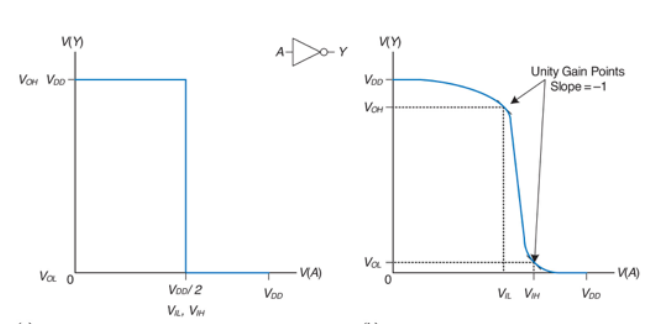
\includegraphics[width=15cm]{TransferChar.png}\\
\begin{itemize}
\item An ideal inverter would output $V_{DD}$ for outputs up to $V_{DD}/2$ and output 0 for inputs above $V_{DD}/2$
\item Real circuits are not ideal
\item A reasonable choice of logic levels is at the points where the slope is -1
\end{itemize}
\subsection{The static Discipline}
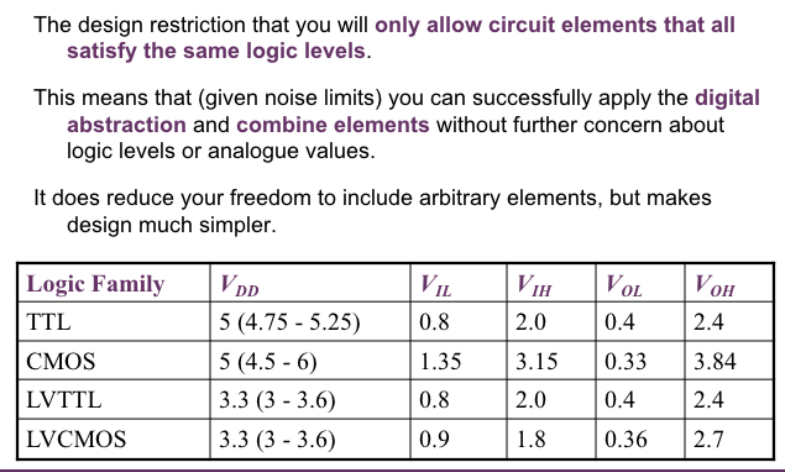
\includegraphics[width=15cm]{StatDis.png}
\section{Moore's Law}
Transistor density doubles in 2 years or computer processing power doubles every 18 months
\end{document}